% !TEX program = lualatex
%==============================================================================
% プリアンブル (Preamble)
%==============================================================================

% ===== ドキュメントクラス =====
% LuaLaTeX向けの日本語縦書きにも対応した標準的なクラス
\documentclass[
  a4paper,
  11pt,
]{ltjsarticle}

%------------------------------------------------------------------------------
% パッケージ読み込み
%------------------------------------------------------------------------------

% ===== フォント・言語設定 (LuaLaTeX専用) =====
\usepackage{luatexja-fontspec} % fontspecを日本語向けに拡張し、モダンなフォントシステムを有効化
% \usepackage{luatexja-preset} % (代替案) システム標準の和文フォントを自動設定する場合に利用

% ===== レイアウト関連 =====
\usepackage[margin=2.5cm]{geometry} % 余白を簡単に設定
\usepackage{graphicx}          % 画像の挿入 (\includegraphics)
\usepackage{booktabs}          % 見栄えの良い表 (\toprule, \midrule, \bottomrule)
\usepackage{float}             % 図表の位置調整 (`[H]`オプション)
\usepackage{wrapfig}           % 文章中への図の回り込み

% ===== 数式・物理単位関連 =====
\usepackage{amsmath}           % 高度な数式環境 (align, pmatrixなど)
\usepackage{amsthm}            % 定理環境 (proofなど)
\usepackage{newtxmath}         % 数式用フォント (Times系)
\usepackage{siunitx}           % 物理単位の記述を統一 (\SI{100}{\ohm})
\usepackage{cancel}            % 数式の打ち消し線 (\cancel)

% ===== 図表・グラフ描画関連 (TikZ/PGF) =====
\usepackage{tikz}
\usepackage{circuitikz}        % 電気回路図の描画
\usepackage{pgfplots}          % 高機能なグラフ描画
\usepackage{pgfplotstable}     % グラフ描画のための表データ操作
\pgfplotsset{compat=1.18}      % pgfplotsのバージョン互換性を保証
\usepgfplotslibrary{statistics} % 統計計算(回帰分析など)ライブラリ
\usetikzlibrary{positioning}   % ノードの相対配置

% ===== プログラミング・アルゴリズム関連 =====
\usepackage{listings}          % ソースコードの表示
\usepackage{algorithm}         % アルゴリズム記述のフロート環境
\usepackage{algpseudocode}     % algorithm環境内で使う疑似コード

% ===== その他 =====
% hyperrefは、原則として最後に読み込むことで他のパッケージとの競合を避ける
\usepackage[
  colorlinks=true,      % リンクに色を付ける
  linkcolor=blue,         % 内部リンクの色 (目次など)
  citecolor=green!60!black, % 参考文献リンクの色
  urlcolor=cyan,          % URLリンクの色
  hidelinks,              % PDF上でリンクの枠を非表示にする (colorlinks=trueと併用推奨)
]{hyperref}

%------------------------------------------------------------------------------
% 各種設定
%------------------------------------------------------------------------------

% ===== フォント設定 =====
% --- 欧文フォント ---
% TeX Liveに標準で同梱されており、環境依存が少ないLatin Modernフォントを指定
\setmainfont{Latin Modern Roman}
\setsansfont{Latin Modern Sans}
\setmonofont{Latin Modern Mono}

% --- 和文フォント ---
% 注意: ご利用の環境にインストールされているフォント名を指定してください。
% 指定したフォントが存在しない場合、コンパイルエラーの原因となります。
% (例: "IPAexMincho", "Noto Serif CJK JP", "Hiragino Mincho ProN")
\setmainjfont[Renderer=HarfBuzz]{Yu Mincho}
\setsansjfont[Renderer=HarfBuzz]{Yu Gothic}
% \setmonojfont[Renderer=HarfBuzz]{Yu Gothic} % 等幅和文フォントが必要な場合

% ===== ドキュメント情報 =====
\title{5. AM}
\author{}
\date{}

% ===== listings (ソースコード) のスタイル設定 =====
\lstset{
  language=Python,
  basicstyle=\small\ttfamily,
  keywordstyle=\color{blue},
  commentstyle=\color{green!50!black},
  stringstyle=\color{purple},
  showstringspaces=false,
  frame=tb,
  captionpos=b,
  breaklines=true,
  numbers=left,
  numberstyle=\tiny\color{gray},
  xleftmargin=2em, % 左側のマージン
  framexleftmargin=1.5em, % フレームと行番号のマージン
}

% ===== pgfplots (グラフ) の共通スタイル設定 =====
\pgfplotsset{
  % レポート内の全グラフに適用する共通スタイルを定義
  report-style/.style={
    xlabel style={yshift=0.5em}, % x軸ラベルと軸の間のスペース
    ylabel style={yshift=-0.5em},% y軸ラベルと軸の間のスペース
    legend pos=north west,
    grid=major,
    ticklabel style={font=\small},
    label style={font=\small},
    legend style={font=\small},
  }
}

% ===== 数式用カスタムコマンド =====
\newcommand{\dd}{\mathrm{d}} % 微分演算子 d
\newcommand{\mi}{\mathrm{j}} % 虚数単位 j

% ===== algorithmicx のスタイル調整 =====
% Procedure をスモールキャピタルではなく太字で表示(フォント警告回避)
\renewcommand{\textproc}[1]{\textbf{#1}}

%==============================================================================
% ドキュメント本体 (Body)
%==============================================================================
\begin{document}

\maketitle

% ===================================================================
\section{目的}
% ===================================================================
AMと復調の原理及びそれを実現する回路の動作を理解する.

% ===================================================================
\section{AMの変調・復調の原理}
% ===================================================================
無線通信では,高い周波数の電磁波を用いなければ,電波の放射が能率よく行われない.そこで,音声のような情報信号をどのようにして高周波にのせるかということが問題となる.その一つの方法がAM変調であり,高周波(搬送波)の振幅を情報信号(変調波)で変化させる方法である.

いま,搬送波 $v_c$ が
\begin{equation}
  v_c = V_c \cos \omega_c t
  \label{eq:carrier}
\end{equation}
で表される正弦波とし,これを
\begin{equation}
  v_s = V_s \cos \omega_s t
  \label{eq:signal}
\end{equation}
で表される信号波(変調波)によって振幅変調する場合を考える.振幅変調は,搬送波の振幅が変調波によって変化する方式なので,被搬送波の振幅は
\begin{equation}
  V_c + k_a V_s \cos \omega_s t
  \label{eq:amplitude}
\end{equation}
となり,振幅が時間によって変化する.ここに,$k_a$ は比例定数である.したがって,被変調波 $v$ は,次のようになる.
\begin{equation}
  v = (V_c + k_a V_s \cos \omega_s t) \cos \omega_c t = V_c(1 + m_a \cos \omega_s t) \cos \omega_c t
  \label{eq:modulated_wave}
\end{equation}
ここで,
\begin{equation}
  m_a = k_a V_s / V_c
  \label{eq:modulation_index}
\end{equation}
であり,これを変調度,または百分率で表して変調率という.

復調は,被変調波を整流または2乗し,それに含まれる低周波成分を取り出すことによってなされる.
振幅変調は,搬送波増幅器の増幅度を変調信号によって変化させればよい.図\ref{fig:waveforms}は変調信号,搬送波及び被変調波である.

\begin{figure}[H]
  \centering
  % 指定されたパスの図を使用
  
\includegraphics[width=0.8\textwidth]{Wave.eps}
  \caption{各部の波形 (a) 変調信号,(b) 搬送波,(c) 被変調波}
  \label{fig:waveforms}
\end{figure}

% ===================================================================
\section{実験}
% ===================================================================
図\ref{fig:circuit}はAM変復調回路である.

\begin{figure}[H]
  \centering
  % 指定されたパスの図を使用
  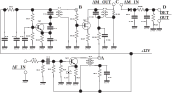
\includegraphics[width=0.9\textwidth]{config.eps}
  \caption{AM 変復調回路}
  \label{fig:circuit}
\end{figure}

\begin{enumerate}
  \item 「AM OUT」端子と「AM IN」端子を接続する.

  \item 低周波発振器を「AF IN」に接続し,\SI{3}{\kilo\hertz}の入力信号に対する図\ref{fig:circuit}の「AF IN」,「AM OUT」及び「DET OUT」端子の電圧波形をスケッチする.ただし,「AM OUT」の包絡線電圧や「DET OUT」が歪まないよう低周波発振器のAmplitudeを調整すること.

  \item \SI{100}{\hertz}~\SI{50}{\kilo\hertz}の周波数範囲の「AF IN」-「AM OUT」及び「DET OUT」間の周波数特性を測定する(10ポイント以上).\\
  注:片対数のグラフ用紙を用いること.「AM OUT」については,包絡線電圧のp-p値を測定すること.

  \item 入力周波数一定としたときの「AF IN」に対する「AM OUT」,「DET OUT」の入出力特性を測定する(10ポイント以上).\\
  注:方眼紙を用いること.「AM OUT」については,包絡線電圧のp-p値を測定すること.
\end{enumerate}

% ===================================================================
\section{考察}
% ===================================================================
\begin{enumerate}
  \item 実験(2)の波形について考察する.
  \item 実験(3)の結果を考察する.
  \item 実験(4)の結果を考察する.
  \item 図\ref{fig:circuit}のAM変復調回路の各部の動作について説明する.
  \item 変調回路及び復調回路を一つずつ調べ動作を説明する.
\end{enumerate}

\end{document}